\documentclass{article}

\usepackage[toc,page]{appendix} \usepackage{amsthm}
\usepackage{amsmath} \usepackage{amssymb} \usepackage{hyperref}
\usepackage{fancyhdr}
\usepackage{graphicx}

\pagestyle{fancy}

\setlength{\parindent}{0pt}

\title{TA Assignment Problem} \author{University of Calgary - CPSC 433
  - Fall 2013\\ \\Carson Tunna, Tyler Smith, Adam Thompson}
\date{October 22, 2013}

\begin{document}

\maketitle\pagebreak

\tableofcontents\pagebreak

\section{Preamble}

For this problem we decided on OR-Tree based search and Set based
search. Our reasoning was as follows. We immediately had a solution
using an OR-Tree based model that covered every combination of TA
assignments to time slots. We figured using a greedy heuristic for our
$altern$ function we could likely come up with an optimal or slightly
sub optimal solution with relative ease. Our second choice as set
based search was very natural in that set based search allows for so
much flexibility. On top of this, the $F_{werth}$ function of set
based search parallels with the soft(and hard) constraints detailed in
the problem description. We were uninspired when we considered the
option of using an AND-Tree based search model simply because it's
difficult to apply a $div$ function to the structure of this problem.
Finally the main reason for selecting these search paradigms was
professor Kremer confirming our instincts and telling us we made the
right choice.

\section{OR-Tree Based Search}
\label{otree}

Let $L$ be the set of all tutorials or labs and $T$ be set of all
TA's. Then the problem is defined as follows:\\

\begin{enumerate}

\item $\forall x \in L$, $\exists y\in T$ such that instructs($y$,
  $l$).
  
\item All hard constraints are satisfied\footnote{See appendix}
  

\end{enumerate}

\subsection{Explanation of Model}

We're looking for an assignment of TA's to labs such that no hard
constraints are violated and as few soft constraints are violated.

The algorithm works as follows

\begin{enumerate}

\item Set the root node to the empty set

\item Pick a lab

\item From the root, draw a branch for every TA that can teach this TA
  without violating any hard constraint.
  

\item Sort the branches from the root node by goodness value in
  ascending order\footnote{Goodness value is calculated by the number
    of soft constraints are currently being violated. The largest
    goodness value possible is 0} 


\item Set the left hand node to be your root node. Remove the last lab
  from your set of working labs. Recurse.

\item When there are no more TA's available the left hand arm of the tree
  is the solution

\item While there is still time available for processing - Go back to
  the root of the tree and this time choose 2nd child of the $root = \emptyset$

\end{enumerate}

\subsection{Mathematical Description of the Model}

Let $L$ be the set of labs\\

Let $L'$ be the set of labs without a TA assignment yet\\

Let $T$ be the set of all TA's\\

Let $I : T \times L$ be a set of ordered pairs representing an
assignment of a TA to a lab.

\subsubsection{Defining the problem instance}

We defined our problem instance as follows

\[
pr = \langle (l_1, t_1), (l_2, t_2), ..., (l_n, t_n)  \rangle
\]

Where $(l_i, t_i) \in I$ and $pr : Prob = sequence$ $I$\\

States can be described by

\[
S = OTree(Prob, \{yes, no, ?\}, b_1 ... b_n)
\]

\subsubsection{Evaluating Solutions}

We define the function $f_{leaf} : S \times Env \rightarrow \mathbb{N}$

\[
f(s) = \sum_{t \in T} Cv(\langle (l_1, t_1) ... (l_n, t_n) \rangle)
\]

Where $Cv: Prob \rightarrow \mathbb{N}$ is a function that takes in a
sequence of assignments and returns the sum of constraints being violated.

\subsubsection{When is a branch solvable or unsolvable}

A $pr$ is unsolvable when

\begin{center}
$Erw_{v,wt}((pr, ?),(pr, no)) \iff (l, t) \in I \land violates-hard-constraint((l,t))$
\end{center}

I.e. for every assignment of a TA to a specific lab, a hard constraint
is violated.\\

A $pr$ is solved when\\

\begin{center}
  $Erw_{v,wt}((pr, ?),(pr, yes)) \iff \lnot Erw_{v,wt}((pr, ?),(pr,
  no)) \land |L'| = \emptyset$

\end{center}

I.e. the problem is not unsolvable and all the labs have been assigned
a TA.

\subsubsection{Branching Definition}

Define $Altern$ in the following way 

\begin{center}
  $Altern(s, s')$ such that $(|s| + 1 = |s'|) \land getLab(last(s')) \in
  L' \land getTA(last(s')) \in T$ 
\end{center}

Where $getLab() : I \times L \rightarrow L$ returns the lab from a
tuple in $I$. Similarly for $getTA()$\\

I.e. the sequence $s'$ is longer than $s$ and we have assigned a TA to a lab
which hasn't had any assignment prior.

\begin{center}
  $Erw((pr, ?), (pr, ?, (pr_1, ?), (pr_2, ?), ... , (pr_n, ?)))$ if $pr_i$
  is generated out of assigning a valid TA to $pr_i$ such that this
  assignment doesn't violate any hard constants
\end{center}


Children are chosen using $f_{trans}$ as follows

\begin{center}
  $Erw((pr, ?, b_1, ... b_n)(pr', ?, b'_1, ... b'_n))$ such that $1
  \leq i \leq n, pr' = min(f_{leaf}(append(pr, b_i)))$
  
\end{center}

\subsection{Demonstration of a small search instance}



\section{Set-Based Search}

\subsection{Explanation of Model}

The Set based search algorithm works as follows.

\begin{enumerate}

\item Start with an initial state $S_0$ of approximately fifty facts.
  This can be generate via random walks of our OR-Tree based tree

\item Take the best fact in $S_0$ and set it to max

\item Modify each fact by swapping TA assignments such that it
  enhances or doesn't change the $f_{wert}$ value of functions

\item Update the value of max

\item While there is still time left, go back to step 3


\end{enumerate}

\subsection{Mathematical Description of the Model}

\subsubsection{Model}

Let $L$ be the set of labs\\

Let $T$ be the set of all TA's\\

Let $I : T \times L$ be a set of ordered pairs rerpresenting an
assignment of a TA to a lab.\\

Let a fact $f \in I$\\

Let $F$ be a set of facts\\

Let a state $S \subseteq 2^F$.\\

Let $A = (S, T)$.\\

Let $T: S \times S$ and $T = \{ (s,s')| \exists A \to B \in Ext \land A
\subseteq s \land s' =(s-A) \cup B \}$ \\

A fact $f$ does not violate hard-constraints given in Appendix \ref{hard}. That is,
\begin{enumerate}
\item No TA has more than \textit{MAX\_LABS} labs: for any fact $f$, $\forall t_i |(t_i,l)\in f|\le MAX\_LABS$.
\item If a TA has a lab, that TA has at least \textit{MIN\_LABS} labs: for any fact $f$, $\forall t_i |(t_i,l)\in f|= 0 \lor |(t_i,l)\in f|\ge MIN\_LABS$
\item No lab has more than one TA and all labs have a TA: for any fact $f$, $\forall l_i |(t, l_i) \in f| = 1$
\item No TA has a time conflict: for any fact $f$, $\forall \left( t_i, l_i \right) \in f, time \left( l_i \right) \notin \lbrace time \left( c_k \right) \land c_k \in courses \left( t_i \right) \rbrace \land time(l_i) \notin \lbrace time(l_j) \land (t_i, l_j) \in f \rbrace $
\end{enumerate}

Define $Ext : \lbrace A \to B | A,B \subseteq F \rbrace$ where $B = A
\cup C$ where $C$ is generated by specifying an allowable time and
calling \textit{Generate} then \textit{Combine} until that time is
exceeded or until $|C| = |A|$ so that $|B| = 2|A|$. The operations
used are defined as:

\begin{enumerate}

\item \textit{Generate} - Do a random walk through the defined in
  \ref{otree}. The random walk does not compare leafs, it only tries
  paths at random until a solution is found. If no solution is found
  within the allowed time, this operation fails.

\item \textit{Combine} - First, map each element in a fact $f$ from a
  2-tuple to a 3-tuple $(t, l) \to (t, l, b = time(l))$. Then, for
  each $b$ such that $\exists (t',l',b) \in f$, match each instance of
  $t'$ and $l'$ once at random. This does not change the times that
  any TA teaches, it only changes which labs a TA is teaching. If the
  result violates any hard constraints, this operation fails. For the
  implementation, we will consider lazy evaluation of hard
  constraints.
\end{enumerate}


\subsubsection{Process}

We define our process $P: (A, Env, K)$ for the set based search. The
model $A$ has already been defined. It is assumed that the environment
$Env$ is unchanging so $K: S \times Env \to S$ is just $K: S \to S$.
The control $K$ for a set based search is defined in Figure \ref{control}.

\begin{figure}
\centering
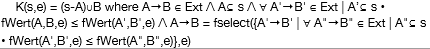
\includegraphics{control}
\caption{\label{control} The control $K$ from the course rubric.}
\end{figure}

$f_{wert}$ is defined as $-\sum\limits_{i}^{} penalty_i(f)$ where $
penalty_i$ is defined in Figure \ref{soft} as a function of a fact
which is either the penalty value from the table or zero if the
penalty does not apply.

$f_{select}$ is defined as a tournament. The number of facts is
``culled'' down to a specified number $N$. This is done by repeating
the following operation $|A|-N$ times. At random, two facts in $f_1,
f_2 \in F$ are selected. A random number $0 < r < 1$ is generated. If
$r < \frac{f_{1wert}}{f_{1wert} + f_{2wert}}$, $f_1$ is removed from
$A$, otherwise $f_2$ is removed from $A$. For the implementation,

\subsection{Demonstration of a small search instance}

\pagebreak
\begin{appendices}

  \section{Hard Constraints}
\label{hard}
  \begin{enumerate}
    
  \item every TA is assigned at most MAX\_LABS labs\\ FORALL ta:TA .
    lab-count(ta) $\leq$ MAX\_LABS)\\

  \item every TA is assigned at least MIN\_LABS labs (if the TA *has* a
    lab assignment)\\ FORALL ta:TA . lab-count(ta) $\not=$ 0 then
    lab-count(ta) $\geq$ MIN\_LABS)\\

  \item  no lab has more than one TA assigned to it\\ FORALL
    course:Course, lab:Lab $|$ has-lab(course,?,lab) . $\lnot$ EXISTS
    ta1,ta2:TA $|$ ta1$\not=$ ta2 . instructs(ta1,lab) $\land$
    instructs(ta2,lab)\\

  \item every lab has a TA assigned to it\\ FORALL course:Course, lab:Lab
    $|$ has-lab(course,?,lab). EXITS ta:TA . instructs(ta,course,lab)\\

  \item no TA is assigned simultaneous labs\\ FORALL ta:TA, c1,c2:Course,
    b1,b2:Lab $|$ (c1=c2 => b1 $\not=$ b2) $\land$ instructs(ta,c1,b1)
    $\land$ instructs(ta,c2,b2) . $\lnot$ EXISTS t1,t2 $|$ at(c1,b1,t1)
    $\land$ at(c2,b2,t2) . conflicts(t1,t2)\\

  \item no TA is assigned a lab that conflicts with his/her own
    courses\\ FORALL ta:TA, course:Course, lab:Lab $|$
    instructs(ta,course,lab) .\\ (($\lnot$ EXISTS c:Course, lec:Lecture
    $|$ taking(ta,c,lec) . EXISTS t1,t2 $|$ at(course,lab,t1) $\land$
    at(c,lec,t2)) . conflicts(t1,t2)) $\land$\\ (($\lnot$ EXISTS
    c:Course, b:Lab $|$ taking(ta,c,b) . EXISTS t1,t2 $|$
    at(course,lab,t1) $\land$ at(c,b,t2)) . conflicts(t1,t2)))\\

    where:\\ lab-count(TA) is a function that returns the number of labs
    a TA instructs.\\

  \end{enumerate}
  
  \section{Soft Constraints}
  \begin{figure}
  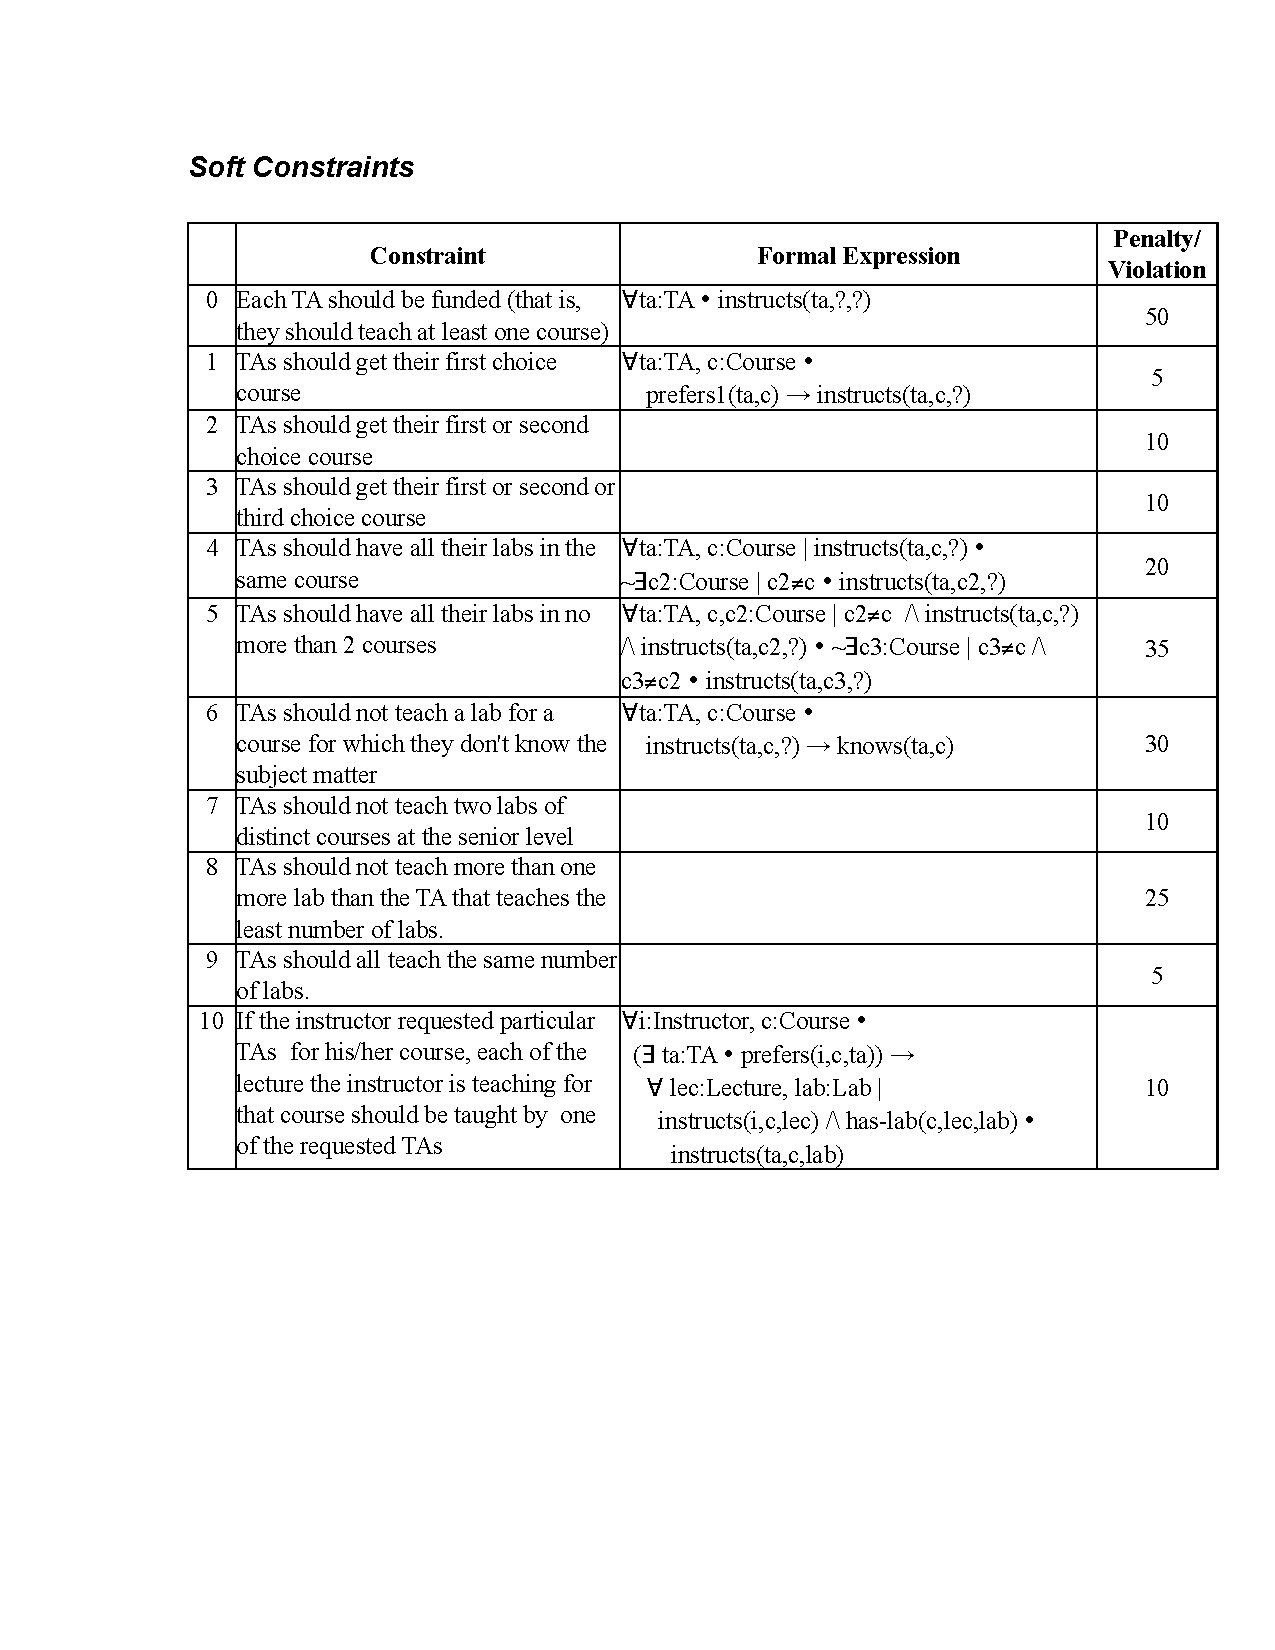
\includegraphics[scale=0.5]{softConstraints}
  \caption{\label{soft}The table of soft constraints with penalties given in the course assignment}
  \end{figure}
  

\end{appendices}

\end{document}
